\subsection{Learning invariant representations}
\label{hsicinvariant}

\begin{figure}

    
    
      \tikzstyle{latent} = [circle,fill=white,draw=black,inner sep=1pt,
minimum size=30pt, font=\fontsize{15}{15}\selectfont, node distance=1]


  \newcommand{\ltkiz}{1cm}
  
  
\captionsetup[subfigure]{justification=centering}
    \centering  
    \begin{subfigure}[t]{0.3\textwidth}
        \centering   
		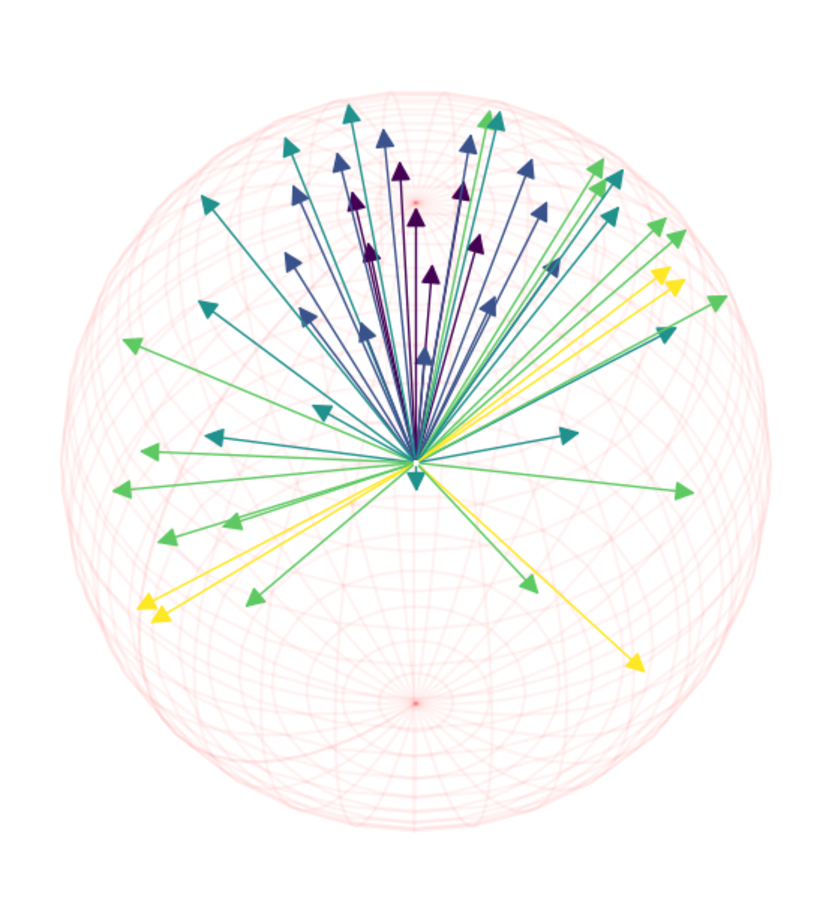
\includegraphics[width=3cm]{figures/angles.pdf}
        \caption{$s$: angle between the camera and the light source}
    \end{subfigure}%
    ~ 
    \begin{subfigure}[t]{0.3\textwidth}
        \centering  
		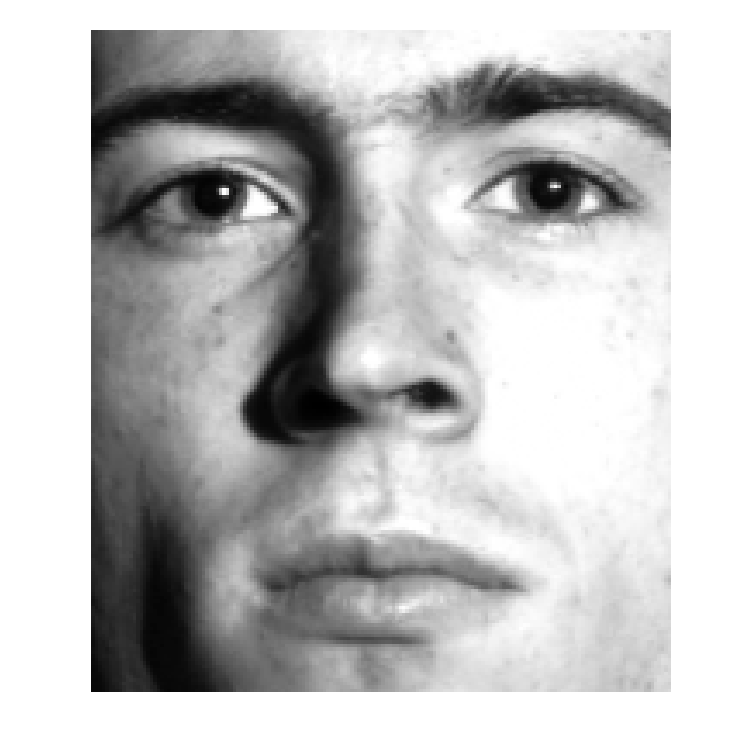
\includegraphics[width=0.7\textwidth]{figures/face.pdf}
        \caption{One image $x$ for a given lighting condition $s$ and person $y$}
    \end{subfigure}
        ~ 
    \begin{subfigure}[t]{0.3\textwidth}
        \centering  
        \scalebox{0.65}
        {
\tikz{ %
  \node[obs] (x) {${x}$} ; %
  \node[obs, above=0.5 * \ltkiz of x, xshift=+1.5\ltkiz] (s) {${s}$};
    \node[latent, above=0.5 * \ltkiz of x,xshift=0*\ltkiz] (z1) {${z_1}$};
      \node[obs, above=0.5 * \ltkiz of z1, xshift=+1.5\ltkiz] (y) {${y}$};
    \node[latent, above=0.5 * \ltkiz of z1,xshift=0*\ltkiz] (z2) {${z_2}$};    
    \edge {z1} {x};
    \edge{z2} {z1};
    \edge {y} {z1};
    \edge {s} {x};
} }
 \caption{Complete graphical model}
    \end{subfigure}
        \caption{Framework for learning invariant representations in the Extended Yale B Face dataset.}
    \label{hsicyale}
\end{figure}


We now consider the particular problem of learning representations for the data that is \emph{invariant} to a given nuisance variable. As a particular instance of the graphical model in Figure~\ref{hsicpgm}b, we embed an image $x$ into a latent vector $z_1$ whose distribution is independent of the observed lighting condition $s$ while being predictive of the person identity $y$ (Figure~\ref{hsicyale}). The generative model is defined in Figure~\ref{hsicyale}c and the variational distribution decomposes as:
\begin{align}
     q_\phi(z^1, z^2 \mid x, s, y) = q_\phi(z^1 \mid x, s)q_\phi(z^2 \mid z^1, y),
\end{align}
as in~\cite{VFAE}. This problem has been studied in~\cite{VFAE} for binary or categorical $s$. For their experiment with a continuous covariate $s$, they discretize $s$ and use the MMD to match the distributions $\hat{q}_\phi(z^1 \mid s=0)$ and $\hat{q}_\phi(z^1 \mid s=j)$ for all $j$. Perhaps surprisingly, their penalty turns out to be a special case of our HSIC penalty.

\begin{thm}
\label{hsicmmd_hsic}
Let the nuisance factor $s$ be a discrete random variable and let $l$ (the kernel for $\mathcal{K}$) be a Kronecker delta function $\delta: (s, s') \mapsto \mathds{1}_{s = s'}$. Then, the V-statistic corresponding to $\textrm{HSIC}
(\hat{q}_\phi(z^1), p_{\text{data}})$ is a weighted sum of the V-statistics of the MMD between the pairs $\hat{q}_\phi(z \mid s=i), \hat{q}_\phi(z \mid s=j)$. The weights are functions of the empirical probabilities for $s$.
\end{thm}
\begin{proof}
     The proof relies on sum manipulations. First, we carefully write the case where $s$ is binary without loss of generality. Let us assume $M$ samples from the joint $(x, s)$ and let us reorder them such that $s_0 = ... = s_N = 0$ and $s_{N+1} = ... = s_M = 1$. In that case,
     
     \begin{align*}
     \begin{split}
          \textrm{HSIC} &=  \frac{1}{M^2}\sum_{ij}^M k_{ij}l_{ij} + \frac{1}{M^4}\sum_{ijkl}^M k_{ij}l_{kl} - \frac{2}{M^3}\sum_{ijk}^M k_{ij}l_{ik} \\ ~ \\
          \textrm{HSIC} &= \frac{1}{M^2}\sum_{i=0}^N\sum_{j=0}^N k_{ij} + \sum_{i=N+1}^M\sum_{j=N+1}^M k_{ij} + \frac{N^2 + (M-N+1)^2}{M^4}\sum_{ij}^M k_{ij} \\
     &- \frac{2}{M^3}\left(N \sum_{i=0}^N \sum_j^M k_{ij} + (M-N+1) \sum_{i=N+1}^M \sum_j^M k_{ij} \right) \\ ~ \\
     \textrm{HSIC} &= \frac{(M-N+1)^2}{M^4} \sum_{i=0, j=0}^Nk_{ij} + \frac{N^2}{M^4} \sum_{i=N+1, j=N+1}^M k_{ij} -2 \frac{N(M-N+1)}{M^4} \sum_{i=0}^N\sum_{j=N+1}^M k_{ij} \\~\\
     \textrm{HSIC} &= \frac{N^2(M-N+1)^2}{M^4} \left( \frac{1}{N^2}\sum_{i=0, j=0}^Nk_{ij} + \frac{1}{(M-N+1)^2} \sum_{i=N+1, j=N+1}^M k_{ij}\right.  \\
     &\qquad\qquad  \left. -2 \frac{1}{N(M-N+1)} \sum_{i=0}^N\sum_{j=N+1}^M k_{ij}\right).
     \end{split}
     \end{align*}
     Above,  the term inside the parenthesis is the V-statistic for the MMD between $q(z \mid  s=0)$ and $q(z \mid s=1)$. In the general case of $s$ discrete, we then have a sum of MMD weighted by the values of the empirical $p(s)$.
     \end{proof}

Working with the HSIC rather than an MMD penalty lets us avoid discretizing $s$. We take into account the whole angular range and not simply the direction of the light. We apply HCV with mean-field AEVB, $Z = \{z^1, z^2\}, X = \{x, y\}, S = \{s\}, \mathcal{Z}_0 = \{z^1\}$ and $\mathcal{S}_0 = \{s\}$.


\paragraph{Dataset}
The extended Yale B dataset~\cite{YALEB} contains cropped faces~\cite{KCLee05} of 38 people under 50 lighting conditions. These conditions are unit vectors in $\mathbb{R}^3$ encoding the direction of the light source and can be summarized into five discrete groups (upper right, upper left, lower right, lower left and front). Following \cite{VFAE}, we use one image from each group per person (total 190 images) and use the remaining images for testing. The task is to learn a representation of the faces that is good at identifying people but has low correlation with the lighting conditions.

\paragraph{Experiment}
We repeat the experiments from the paper introducing the variational fair auto-encoder (VFAE)~\cite{VFAE}, this time comparing the VAE~\cite{AEVB} with no covariate $s$, the VFAE~\cite{VFAE} with observed lighting direction groups (five groups), and the HCV with the lighting direction vector (a three-dimensional vector). As a supplemental baseline, we also report results for the unconstrained VAEs. As in~\cite{VFAE}, we report 1) the accuracy for classifying the person based on the variational distribution $q_\phi(y \mid z^1, s)$; 2) the classification accuracy for the lighting group condition (five-way classification) based on a logistic regression and a random forest classifier on a sample from the variational posterior $q_\phi(z^1 \mid z^2, y, s)$ for each datapoint; and 3) the average error for predicting the lighting direction with linear regression and a random forest regressor, trained on a sample from the variational posterior $q_\phi(z^1 \mid z^2, y, s)$. Error is expressed in degrees. $\lambda$ is optimized via grid search as in~\cite{VFAE}. 

We report our results in Table~\ref{hsicYale}. As expected, adding information (either the lightning group or the refined lightning direction) always improves the quality of the classifier $q_\phi(y \mid z^1, s)$. This can be seen by comparing the scores between the vanilla VAE and the unconstrained algorithms. However, by using side information $s$, the unconstrained models yield a representation less suitable because it is more correlated with the nuisance variables. There is therefore a trade-off between correlation to the nuisance and performance. Our proposed method (HCV) shows greater invariance to lighting direction while accurately predicting people's identities.


\begin{table}[ht]
\centering
\begin{small}
\begin{tabular}{lccccc}
\toprule
     & \multirow{2}{*}{\begin{tabular}[c]{@{}c@{}}\vspace{-0.1cm}\\ \textbf{Person identity}\\ \textbf{(Accuracy)}\end{tabular}} & \multicolumn{2}{c}{\begin{tabular}[c]{@{}c@{}}\textbf{Lighting group}\\ \textbf{(Average classification error)}\end{tabular}}                                             & \multicolumn{2}{c}{\begin{tabular}[c]{@{}c@{}}\textbf{Lighting direction}\\ \textbf{(Average error in degree)}\end{tabular}}                       \\[0.2 cm]
     &                                                                                       & \begin{tabular}[c]{@{}c@{}}\textbf{Random Forest}\\ \textbf{Classifier}\end{tabular} & \begin{tabular}[c]{@{}c@{}}\textbf{Logistic} \\ \textbf{Regression}\end{tabular} & \begin{tabular}[c]{@{}c@{}}\textbf{Random Forest}\\ \textbf{Regressor}\end{tabular} & \begin{tabular}[c]{@{}c@{}}\textbf{Linear} \\ \textbf{Regression}\end{tabular} \\
     \midrule
\textbf{VAE}  & 0.72                                                                                  & 0.26                                                               & 0.11                                                           & 14.07                                                             & 9.40                                                         \\
\textbf{VFAE}$^*$ & 0.74                                                                                  & 0.23                                                               & 0.01                                                           & 13.96                                                             & 8.63                                                        \\
\textbf{VFAE} & 0.69                                                                                  & 0.51                                                               & \textbf{0.42}                                                           & 23.59                                                             & 19.89                                                        \\
\textbf{HCV}$^*$  & \textbf{0.75}                                                                                  & 0.25                                                               & 0.10                                                           & 12.25                                                             & 2.59 \\
\textbf{HCV}  & \textbf{0.75}                                                                                  & \textbf{0.52}                                                               & 0.29                                                           & \textbf{36.15}                                                             & \textbf{28.04} \\
\bottomrule
\end{tabular}
\end{small}
\caption[Results on the Extended Yale B dataset]{Results on the Extended Yale B dataset. Preprocessing differences likely explain the slight deviation in scores from~\cite{VFAE}. Stars ($^*$) the unconstrained version of the algorithm was used.}
\label{hsicYale}
\end{table}
%\end{wraptable}
